\documentclass{article}

\usepackage{fancyhdr}
\usepackage{extramarks}
\usepackage{amsmath}
\usepackage{amsthm}
\usepackage{amsfonts}
\usepackage{tikz}
\usepackage[plain]{algorithm}
\usepackage{algpseudocode}
\usepackage{color}
\usepackage{listings}
\usepackage{fontspec}

\newfontfamily\menlo{Menlo}
% \newfontfamily\menlo{Consolas}
\lstset{
    columns=fixed,       
    numbers=left,                                        % 在左侧显示行号
    numberstyle=\tiny\color{gray},                       % 设定行号格式
    frame=none,                                          % 不显示背景边框
    backgroundcolor=\color[RGB]{245,245,244},            % 设定背景颜色
    keywordstyle=\color[RGB]{40,40,255},                 % 设定关键字颜色
    numberstyle=\footnotesize\color{darkgray},           
    commentstyle=\it\color[RGB]{0,96,96},                % 设置代码注释的格式
    stringstyle=\rmfamily\slshape\color[RGB]{128,0,0},   % 设置字符串格式
    showstringspaces=true,                              % 不显示字符串中的空格
    numberstyle=\small\menlo,
    basicstyle=\small\menlo,
    breaklines=true,
}

% \lstset{
%     language=Octave,                % the language of the code
%     basicstyle=\footnotesize,           % the size of the fonts that are used for the code
%     numbers=left,                   % where to put the line-numbers
%     numberstyle=\tiny\color{gray},  % the style that is used for the line-numbers
%     stepnumber=1,                   % the step between two line-numbers. If it's 1, each line 
%                                     % will be numbered
%     numbersep=5pt,                  % how far the line-numbers are from the code
%     backgroundcolor=\color{white},      % choose the background color. You must add \usepackage{color}
%     showspaces=false,               % show spaces adding particular underscores
%     showstringspaces=false,         % underline spaces within strings
%     showtabs=false,                 % show tabs within strings adding particular underscores
%     frame=single,                   % adds a frame around the code
%     rulecolor=\color{black},        % if not set, the frame-color may be changed on line-breaks within not-black text (e.g. commens (green here))
%     tabsize=2,                      % sets default tabsize to 2 spaces
%     captionpos=b,                   % sets the caption-position to bottom
%     breaklines=true,                % sets automatic line breaking
%     breakatwhitespace=false,        % sets if automatic breaks should only happen at whitespace
%     title=\lstname,                 % show the filename of files included with \lstinputlisting;
%                                     % also try caption instead of title
%     keywordstyle=\color{blue},          % keyword style
%     commentstyle=\color{dkgreen},       % comment style
%     stringstyle=\color{mauve},         % string literal style
%     escapeinside={\%*}{*)},            % if you want to add LaTeX within your code
%     morekeywords={*,...}               % if you want to add more keywords to the set
% }

\usetikzlibrary{automata,positioning}

%
% Basic Document Settings
%
%%% page layout
\topmargin=-0.45in
\evensidemargin=0in
\oddsidemargin=0in
\textwidth=6.5in
\textheight=9.0in
\headsep=0.25in

\linespread{1.1}    %%% line spacing

\definecolor{ustcblue}{cmyk}{1,0.8,0,0}

\pagestyle{fancy}
\lhead{\hmwkAuthorName}
\chead{\hmwkClass\ (\hmwkClassInstructor): \hmwkTitle}
\rhead{}
\lfoot{}
\cfoot{\thepage}

\renewcommand\headrulewidth{0.4pt}
\renewcommand\footrulewidth{0.4pt}

\setlength\parindent{0pt}

%
% Create Problem Sections
%

\newcommand{\enterProblemHeader}[1]{
    \nobreak\extramarks{}{Problem \arabic{#1} continued on next page\ldots}\nobreak{}
    \nobreak\extramarks{Problem \arabic{#1} (continued)}{Problem \arabic{#1} continued on next page\ldots}\nobreak{}
}

\newcommand{\exitProblemHeader}[1]{
    \nobreak\extramarks{Problem \arabic{#1} (continued)}{Problem \arabic{#1} continued on next page\ldots}\nobreak{}
    \stepcounter{#1}
    \nobreak\extramarks{Problem \arabic{#1}}{}\nobreak{}
}

\setcounter{secnumdepth}{0}
\newcounter{partCounter}
\newcounter{homeworkProblemCounter}
\setcounter{homeworkProblemCounter}{1}
\nobreak\extramarks{Problem \arabic{homeworkProblemCounter}}{}\nobreak{}

%
% Homework Problem Environment
%
% This environment takes an optional argument. When given, it will adjust the
% problem counter. This is useful for when the problems given for your
% assignment aren't sequential. See the last 3 problems of this template for an
% example.
%
\newenvironment{homeworkProblem}[1][-1]{
    \ifnum#1>0
        \setcounter{homeworkProblemCounter}{#1}
    \fi
    \subsection{Exercise \arabic{homeworkProblemCounter}}
    \setcounter{partCounter}{1}
    \enterProblemHeader{homeworkProblemCounter}
}{
    \exitProblemHeader{homeworkProblemCounter}
}

%
% Homework Details
%   - Title
%   - Due date
%   - Class
%   - Section/Time
%   - Instructor
%   - Author
%

\newcommand{\hmwkTitle}{Homework\ \#3}
\newcommand{\hmwkDueDate}{\today}
\newcommand{\hmwkClass}{Inversion}
\newcommand{\hmwkClassInstructor}{Professor H. Yao \& H. Zhang}
\newcommand{\hmwkAuthorName}{\textbf{Jintao Li}}
\newcommand{\hmwkAuthorID}{\textbf{SA20007037}}
\newcommand{\hmwkAuthoremail}{\textbf{E-mail: lijintao@mail.ustc.edu.cn}}

%
% Title Page
%

% \title{
%     \vspace{2in}
%     \textbf{\hmwkClass:\ \hmwkTitle}\\
%     \normalsize\vspace{0.2in}\large{\hmwkDueDate}\\
%     \vspace{0.2in}\large{\textit{\hmwkClassInstructor}}
%     \vspace{3in}
% }

% \author{\hmwkAuthorName \\
% \hmwkAuthorID}
% \date{}

\renewcommand{\part}[1]{\textbf{ \\ (\alph{partCounter})  }\stepcounter{partCounter} }

%
% Various Helper Commands
%

% Useful for algorithms
\newcommand{\alg}[1]{\textsc{\bfseries \footnotesize #1}}

% For derivatives
\newcommand{\deriv}[1]{\frac{\mathrm{d}}{\mathrm{d}x} (#1)}

% For partial derivatives
\newcommand{\pderiv}[2]{\frac{\partial}{\partial #1} (#2)}

% Integral dx
\newcommand{\dx}{\mathrm{d}x}

% Alias for the Solution section header
\newcommand{\solution}{\textbf{\large \\ Solution: \\}}

% Probability commands: Expectation, Variance, Covariance, Bias
\newcommand{\E}{\mathrm{E}}
\newcommand{\Var}{\mathrm{Var}}
\newcommand{\Cov}{\mathrm{Cov}}
\newcommand{\Bias}{\mathrm{Bias}}

%
\newcommand{\mb}[1]{\mathbf{#1}}

\begin{document}

\begin{titlepage}

\begin{center}

\textcolor{ustcblue}{
\includegraphics[width=0.25\textwidth]{./ustc_logo_fig.pdf} \\ [1cm]}
% Title
{ \Huge \bfseries \hmwkClass\ \hmwkTitle}\\[1cm]

\large \textbf{\hmwkClassInstructor} \\ [5cm]

\large \hmwkAuthorName \\ [0.25cm]
\large \hmwkAuthorID \\ [0.25cm]
\large \hmwkAuthoremail
\vfill
% Bottom of the page
{\large \today}

\end{center}

\end{titlepage}

\begin{center}
\section{Chapter 2}
\end{center}

\begin{homeworkProblem}[1]
A seismic profiling experiment is performed where the first arrival times of seismic
energy from a mid-crustal refractor are observed at distances (in kilometers) of 
\begin{equation}
    \mb{x} = \left[ \begin{matrix}
        6.0000 \\ 10.1333 \\ 14.2667 \\ 18.4000 \\ 22.5333 \\ 26.6667
    \end{matrix} \right]
\end{equation}

from the source, and are found to be (in seconds after the source origin time)
\begin{equation}
    \mb{t} = \left[ \begin{matrix}
        3.4935 \\ 4.2853 \\ 5.1374 \\ 5.8181 \\ 6.8632 \\ 8.1841 
    \end{matrix} \right] .
\end{equation}

These vectors can also be found in the MATLAB data file \textbf{profile.mat}. 
A two-layer, flat Earth structure gives the mathematical model
\begin{equation}
    t_i = t_0 + s_2 x_i ,
\end{equation}

where the intercept time, $t_0$, depends on the thickness and slowness of 
the upper layer, and $s_2$ is the slowness of the lower layer. The estimated 
noise in the first arrival time measurements is believed to be independent 
and normally distributed with expected value $0$ and standard deviation 
$\sigma = 0.1 s$. 

\textbf{matlab code: prepare profile.mat}
\begin{lstlisting}[language={matlab}]
x = [6.0000 10.1333 14.2667 18.4000 22.5333 26.6667]';
t = [3.4935 4.2853 5.1374 5.8181 6.8632 8.1841]';
save("profile.mat", "x", "t")
\end{lstlisting}



\part

Find the least squares solution for the model parameters $t_0$ and $s_2$. Plot the data,
the fitted model, and the residuals. 

\solution

\begin{equation}
    \mb{m}_{L_2} = \left[\begin{matrix} t_0 \\ s_2
    \end{matrix}\right]
    = (\mb{G}^T \mb{G})^{-1} \mb{G}^T \mb{t} = 
    \left[\begin{matrix}
        2.0323 \\ 0.2203
    \end{matrix}\right] ,
\end{equation}

where 

\begin{equation}
    \mb{G} = \left[ \begin{matrix}
        1 & x_1 \\ 1 & x_2 \\ 1 & x_3 \\ 1 & x_4 \\ 1 & x_5 \\ 1 & x_6
    \end{matrix} \right] .
\end{equation}

\textbf{matlab code}
\begin{lstlisting}[language={matlab}]
clear;clc;close all;
load("profile.mat")

G = [ones(6, 1), x];
m_L2 = inv(G' * G) * G' * t;
r = t - G * m_L2;

% plot the data, the fitted model
figure(1)
plot(x, t, "ro");
hold on;
t_m = G * m_L2;
plot(x, t_m, "-b");
xlabel("Distances/km");
ylabel("The first arrival times/s")
legend(["data", "the fitted model"], "Location", "southeast")

% plot the residual
figure(2)
plot(x, r, "-o");
xlabel("Distances/km");
ylabel("The differece of times/s")
title("The residual")
\end{lstlisting}

\begin{figure}[htb]
    \centering
    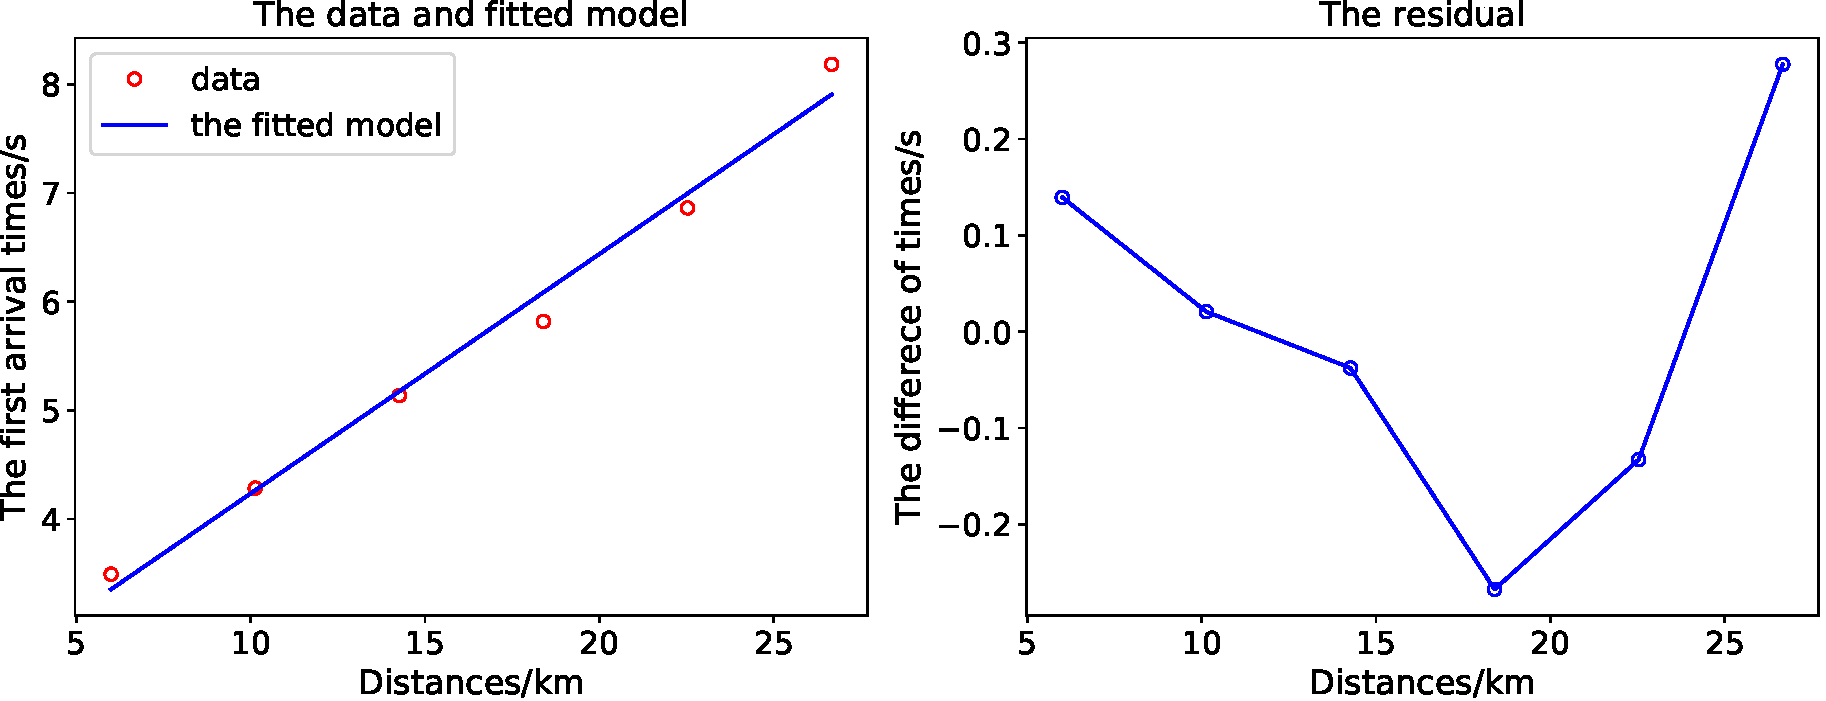
\includegraphics[width=6in, keepaspectratio]{hw3/hw3e1a.pdf}
    \label{fig:hw3e1a}
\end{figure}


\part

Calculate and comment on the model parameter correlation matrix (e.g., 2.43).
How are the correlations manifested in the general appearance of the error
ellipsoid in $(t_0, s_0)$ space? 

\solution

\begin{equation}
    \mb{Cov}(\mb{m}_{L_2}) = \sigma^2 (\mb{G}^T\mb{G})^{-1}
\end{equation}

\begin{equation}
    \rho_{m_{i}, m_{j}}=\frac{\operatorname{Cov}\left(m_{i}, m_{j}\right)}{\sqrt{\operatorname{Var}\left(m_{i}\right) \cdot \operatorname{Var}\left(m_{j}\right)}}
\end{equation}
So, 
\begin{equation}
    \mb{\rho} = \left[ \begin{matrix}
        1 & -0.9179 \\ -0.9179 & 1
    \end{matrix} \right]
\end{equation}

\textbf{matlab code}
\begin{lstlisting}[language={matlab}]
%% 1-b
Sigma = 0.1;
C = Sigma^2 .* inv(G' * G);
rho = C(1,2) ./ sqrt(C(1,1) .* C(2,2));
correlation_matrix = [1 rho; rho 1];
\end{lstlisting}


\part

Plot the error ellipsoid in the $(t_0, s_2)$ plane and calculate conservative 
$95\%$confidence intervals for $t_0$ and $s_2$ for the appropriate value of $\Delta^2$. 
Hint: The following MATLAB function will plot a two-dimensional covariance 
ellipse about the model parameters, where C is the covariance matrix, 
DELTA2 is $\Delta^2$, and $m$ is the 2-vector of model parameters. 

\textbf{matlab code}
\begin{lstlisting}[language={matlab}]
%set the number of points on the ellipse to generate and plot
function plot_ellipse(DELTA2,C,m)
n=100;
%construct a vector of n equally-spaced angles from (0,2*pi)
theta=linspace(0,2*pi,n)';
%corresponding unit vector
xhat=[cos(theta),sin(theta)];
Cinv=inv(C);
%preallocate output array
r=zeros(n,2);
for i=1:n
    %store each (x,y) pair on the confidence ellipse
    %in the corresponding row of r
    r(i,:)=sqrt(DELTA2/(xhat(i,:)*Cinv*xhat(i,:)'))*xhat(i,:);
end
plot(m(1)+r(:,1), m(2)+r(:,2));
axis equal
\end{lstlisting} 

\solution

The degrees of freedom is 2, so $\Delta^2 = 5.99$.
And the eigenvalues of $\mb{C}^{-1}$ is 
\begin{equation}
    \left[\lambda_{1}, \lambda_{2}\right] \approx[90, 190470] .
\end{equation}
So, 
\begin{equation}
    \sqrt{F_{\chi^{2}, 3}^{-1}(0.95)}\left[1 / \sqrt{\lambda_{1}}, 
    1 / \sqrt{\lambda_{2}}\right] \approx[238,1068.1]
\end{equation}

i.e.

\begin{equation}
    \left[t_0, s_2\right] = \left[2.0323\pm238, 0.2203\pm1068.1\right]
\end{equation}

The error ellipsoid in the $(t_0, s_2)$ plane:

\begin{figure}[htb]
    \centering
    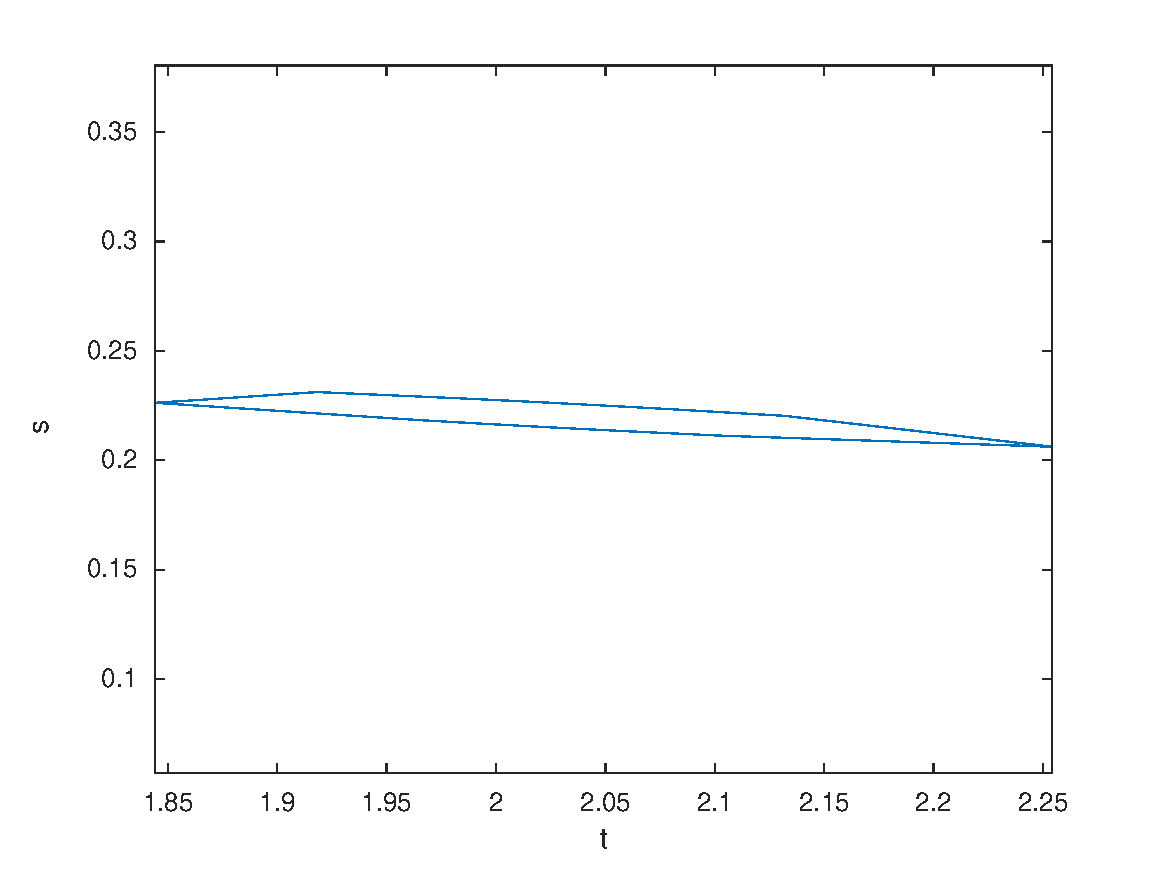
\includegraphics[width=6in, keepaspectratio]{hw3/hw3e1c.pdf}
    \label{fig:hw3e1c}
\end{figure}

\textbf{matlab code}
\begin{lstlisting}[language={matlab}]
%% 1-c
DeltaS = 5.99;
plot_ellipse(DeltaS, C, m_L2)
xlabel("t_0 / s")
ylabel("s_2 / km")
lambda = eig(inv(C));
intv = sqrt(DeltaS) .* lambda .^ 0.5;
\end{lstlisting} 


\part

Evaluate the \textit{p}-value for this model. You may find the library function 
\textbf{chi2cdf} to be useful here. 

\solution

The $\chi^2$ value for this regression is :
\begin{equation}
    \chi_{obs}^2 = \sum\limits_{i=1}^m (t_i - (\mb{Gm}_{L_2})_i)^2 / \sigma_i^2 .
\end{equation}

And using matlab \textbf{chi2cdf} to calculate the \textit{p}-value, 
which is $8.7992\times 10^{-4}$

\textbf{matlab code}
\begin{lstlisting}[language={matlab}]
%% 1-d
chiValue = sum(r.^2 ./ Sigma^2);
p = chi2cdf(chiValue, 4, "upper");
\end{lstlisting}

\part

Evaluate the value of $\chi^2$ for 1000 Monte Carlo simulations using the data 
prediction from your model perturbed by noise that is consistent with the data
assumptions. Compare a histogram of these $\chi^2$ values with the theoretical 
$\chi^2$ distribution for the correct number of degrees of freedom. You may 
find the library function \textbf{chi2pdf} to be useful here. 

\solution

\textbf{matlab code}
\begin{lstlisting}[language={matlab}]
%% 1-e
chi_sim = zeros(1, 1000);
p_sim = zeros(1, 1000);
for i = 1:1:1000
    noise = 0.1*randn(6, 1);
    t_noise = t + noise;
    m_noise = inv(G' * G) * G' * t_noise;
    r = t_noise - G * m_noise;
    chiv = sum(r .^2 ./ Sigma^2);
    chi_sim(i) = chi2cdf(chiv, 4);
    p_sim(i) = chi2cdf(chiv, 4,"upper");
end

histogram(chi_sim-chi);
\end{lstlisting}

\begin{figure}[htb]
    \centering
    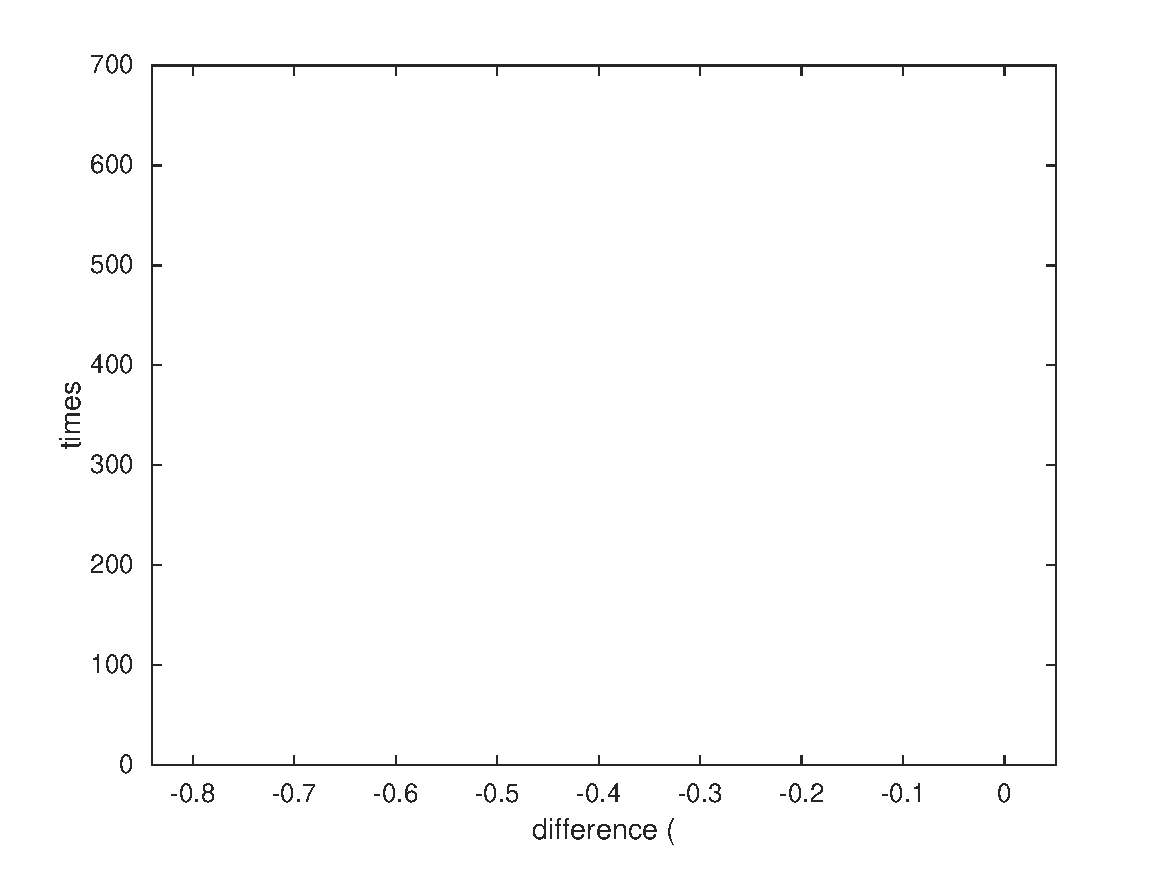
\includegraphics[width=6in, keepaspectratio]{hw3/hw3e1e.pdf}
    \label{fig:hw3e1e}
\end{figure}



\part

Are your \textit{p}-value and Monte Carlo $\chi^2$ distribution consistent 
with the theoretical modeling and the data set? If not, explain what is wrong.

\solution
\textbf{matlab code}
\begin{lstlisting}[language={matlab}]
%% 1-f
histogram(p_sim-p);
\end{lstlisting}

\begin{figure}[htb]
    \centering
    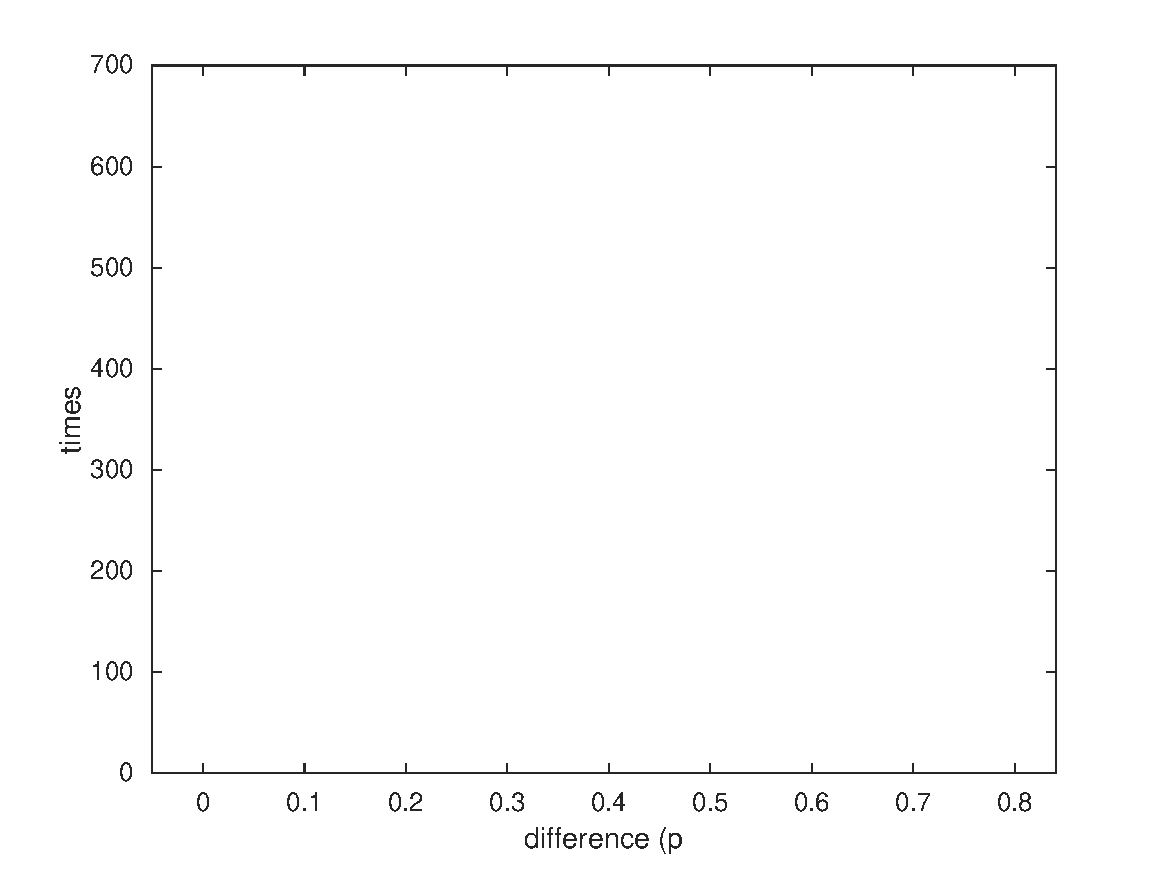
\includegraphics[width=6in, keepaspectratio]{hw3/hw3e1f.pdf}
    \label{fig:hw3e1f}
\end{figure}

\part

Use IRLS to find 1-norm estimates for $t_0$ and $s_2$. Plot the data 
predictions from your model relative to the true data and compare with (a). 

\solution

We set the iteration tolerance $\tau = 0.0001$ and $\epsilon = 0.0001$.

\textbf{matlab code: create IRLS.m, which performs IRLS.}
\begin{lstlisting}[language={matlab}]
function m = IRLS(t, G)

condition = true;
threshold = 0.0001;
epsilon = 0.0001;

m0 = inv(G' * G) * G' * t;

r = abs(t - G * m0);
r(r < epsilon) = epsilon;
R = diag(r.^-1);

i = 0;
while condition
    i = i+1;
    m1 = (G' * R * G) \ (G' * R * t);
    condition = (norm(m1 - m0) ./ (1 + norm(m1))) > threshold;
    m0 = m1;
    r = abs(t - G * m0);
    r(r < epsilon) = epsilon;
    R = diag(r.^-1);
end

m = m0;
\end{lstlisting}

\textbf{matlab code: find 1-norm estimates }
\begin{lstlisting}[language={matlab}]
load("profile.mat")
G = [ones(6, 1), x];
m_L2 = inv(G' * G) * G' * t;

% plot 2-norm solution
figure(1)
plot(x, t, "ro");
hold on;
t_m = G * m_L2;
plot(x, t_m, "-b");
hold on;

% calculate 1-norm solution and plot it
m_L1 = IRLS(t, G);
plot(x, G * m1, "--g");

xlabel("Distances/km");
ylabel("The first arrival times/s")
legend(["data", "L2 solution", "IRLS"], "Location", "southeast")
\end{lstlisting}

The comparision:

\begin{figure}[htb]
    \centering
    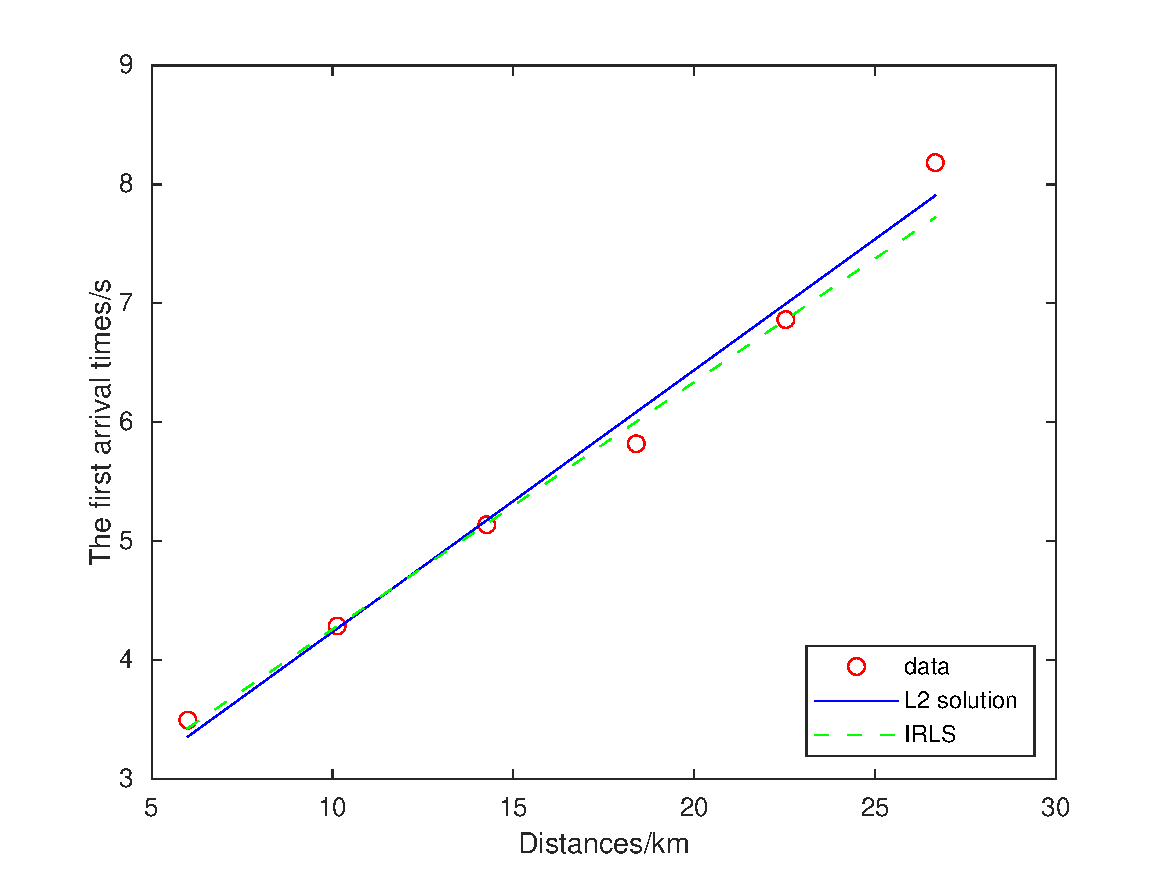
\includegraphics[width=6in, keepaspectratio]{hw3/hw3e1g.pdf}
    \label{fig:hw3e1g}
\end{figure}



\part

Use Monte Carlo error propagation and IRLS to estimate symmetric $95\%$
confidence intervals on the 1-norm solution for $t_0$ and $s_2$. 

\solution

The $95\%$ confidence intervals are given by
\begin{equation}
    \mathbf{m}_{L_{1}} \pm 1.96 \operatorname{diag}
    \left(\operatorname{Cov}\left(\mathbf{m}_{L_{1}}\right)\right)^{1 / 2}.
\end{equation}

And 
\begin{equation}
    \operatorname{Cov}(\mathbf{m}_{L_{1}})= \frac{\mb{A}^T \mb{A}}{q}.
\end{equation}

Calculate it by MATLAB, $\left[ t_0, s_2 \right] = [2.1786\pm0.2996, 0.2079\pm0.0201]$

\textbf{matlab code}
\begin{lstlisting}[language={matlab}]
%% 1-h
q = 1000;
m_all = zeros(q, 2);
A = zeros(q, 2);

for i = 1:1:q
    noise = Sigma .* randn(6, 1);
    t_noise = t + noise;
    m_all(i, :) = (IRLS(t_noise, G))';
end

A = m_all - mean(m_all);

CovML1 = A' * A ./ q;

conf = 1.96 .* diag(CovML1) .^ 0.5;
\end{lstlisting}


\part

Examining the contributions from each of the data points to the 1-norm misfit
measure, can you make a case that any of the data points are statistical outliers? 

\solution





\end{homeworkProblem}

\begin{homeworkProblem}[2]
In this chapter we have largely assumed that the data errors are independent. Suppose
instead that the data errors have an MVN distribution with expected value \textbf{0} and a
covariance matrix $\mb{C}_D$. It can be shown that the likelihood function is then

\begin{equation}
    L(\mathbf{m} \mid \mathbf{d})=\frac{1}{(2 \pi)^{m / 2}} 
    \frac{1}{\sqrt{\operatorname{det}\left(\mathbf{C}_{D}\right)}} 
    e^{-(\mathbf{G} \mathbf{m}-\mathbf{d})^{T} \mathbf{C}_{D}^{-1}
    (\mathbf{G} \mathbf{m}-\mathbf{d}) / 2} .
\end{equation} 

\part

Show that the maximum likelihood estimate can be obtained by solving the
minimization problem,
\begin{equation}
    \min (\mathbf{G m}-\mathbf{d})^{T} \mathbf{C}_{D}^{-1}(\mathbf{G m}-\mathbf{d}) .
\end{equation} 


\solution

\begin{equation}
    \begin{aligned}
    \max \  L(\mb{m}|\mb{d}) 
    & = \max \  e^{-(\mb{Gm}-\mb{d})^T\mb{C}_D^{-1}(\mb{Gm}-\mb{d})/2} \\
    & = \max \  -(\mb{Gm}-\mb{d})^T\mb{C}_D^{-1}(\mb{Gm}-\mb{d})/2 \\
    & = \min \  (\mb{Gm}-\mb{d})^T\mb{C}_D^{-1}(\mb{Gm}-\mb{d}) .
    \end{aligned}
\end{equation}

\part

Show that (2.111) can be solved using the system of equations

\begin{equation}
    \mathbf{G}^{T} \mathbf{C}_{D}^{-1} \mathbf{G} \mathbf{m}=
    \mathbf{G}^{T} \mathbf{C}_{D}^{-1} \mathbf{d} .
\end{equation} 

\solution

To find a solution $\mb{m}$ satisfing (2.111), we can leverage 
its derivative is equal to 0, i.e. 
\begin{equation}
    \begin{aligned}
    & F = (\mb{Gm}-\mb{d})^T\mb{C}_D^{-1}(\mb{Gm}-\mb{d}) \\
    & \frac{\partial F}{\partial \mb{m}} = 0 \\
    \Rightarrow & \mb{G}^T \mb{C}_D^{-1} (\mb{Gm}-\mb{d}) + 
    (\mb{Gm}-\mb{d})^T \mb{C}_D^{-1} \mb{G} = 0 \\
    \Rightarrow & \mb{G}^T \mb{C}_D^{-1} (\mb{Gm}-\mb{d}) = 
    -(\mb{G}^T \mb{C}_D^{-1} (\mb{Gm}-\mb{d}))^T \\
    \Rightarrow & \mb{G}^T \mb{C}_D^{-1} (\mb{Gm}-\mb{d}) = 0 \\
                        i.e. \\
    & \mb{G}^T \mb{C}_D^{-1} \mb{Gm} = \mb{G}^T \mb{C}_D^{-1} \mb{d}
    \end{aligned}
\end{equation}

Note that : $\mb{C}^T = \mb{C}$, so $(\mb{C}^{-1})^T = \mb{C}^{-1}$


\part

Show that (2.111) is equivalent to the linear least squares problem

\begin{equation}
    \min \left\|\mathbf{C}_{D}^{-1 / 2} \mathbf{G m}-
    \mathbf{C}_{D}^{-1 / 2} \mathbf{d}\right\|_{2} ,
\end{equation}

where $\mb{C}_D^{-1/2}$ is the matrix square root of $\mb{C}_D^{-1}$. 


\solution

From the normal equations (A.73), a linear least squares problem can convert
to solve:
\begin{equation}
    \mb{G}^T\mb{Gm} = \mb{G}^T\mb{d} .
\end{equation}

So, the linear least squares problem 
\begin{equation}
    \min \left\|\mathbf{C}_{D}^{-1 / 2} \mathbf{G m}-
    \mathbf{C}_{D}^{-1 / 2} \mathbf{d}\right\|_{2} ,
\end{equation}
can convert to solve :

\begin{equation}
    \begin{aligned}
    & (\mb{C}_D^{-\frac{1}{2}}\mb{G})^T(\mb{C}_D^{-\frac{1}{2}}\mb{G})\mb{m} = 
    (\mb{C}_D^{-\frac{1}{2}}\mb{G})^T\mb{C}_D^{-\frac{1}{2}}\mb{d} \\
    \Rightarrow & \mb{G}^T\mb{C}_D^{-\frac{1}{2}}\mb{C}_D^{-\frac{1}{2}}\mb{G}\mb{m} = 
    \mb{G}^T\mb{C}_D^{-\frac{1}{2}}\mb{C}_D^{-\frac{1}{2}}\mb{d} \\
    \Rightarrow & \mb{G}^T\mb{C}_D^{-1}\mb{G}\mb{m} = 
    \mb{G}^T \mb{C}_D^{-1} \mb{d}
    \end{aligned}
\end{equation}

The two problem can convert to solve a same equation, so the two problem 
are equivalent.


\part

The Cholesky factorization of $\mb{C}_D^{-1}$ can also be used instead of 
the matrix square root. Show that (2.111) is equivalent to the linear least 
squares problem 

\begin{equation}
    \min \|\mathbf{R} \mathbf{G} \mathbf{m}-\mathbf{R} \mathbf{d}\|_{2}
\end{equation}

where $\mb{R}$ is the Cholesky factor of $\mb{C}_D^{-1}$.


\solution



\end{homeworkProblem}

\begin{homeworkProblem}[5]
Use linear regression to fit a polynomial of the form 
\begin{equation}
    y_{i}=a_{0}+a_{1} x_{i}+a_{2} x_{i}^{2}+\ldots+a_{19} x_{i}^{19}
\end{equation}
to the noise-free data points
\begin{equation}
    \left(x_{i}, y_{i}\right)=(-0.95,-0.95),(-0.85,-0.85), \ldots,(0.95,0.95)
\end{equation}
Use the normal equations to solve the least squares problem.

Plot the data and your fitted model, and list the parameters, $a_i$, obtained in your
regression. Clearly, the correct solution has $a_1 = 1$, and all other $a_i = 0$. 
Explain why your answer differs.

\solution
\textbf{matlab code}
\begin{lstlisting}[language={matlab}]
clear;clc;close all;

x = (-0.95:0.1:0.95)';
y = x;

G = zeros(20,20);
for i=1:20
    G(:, i) = x.^(i-1);
end

m = G \ y;
m_true = zeros(20, 1);
m_true(2) = 1;
y_pre = G*m;

figure(1)
plot(x, y, "ro")
hold on;
plot(x, y_pre, "-b")
xlabel("x")
ylabel("y")
legend(["the data", "the fitted model"], "Location", "southeast")

figure(2)
r = m - m_true;
a = 0:1:19;
plot(a, r, "-o")
xlabel("a")
ylabel("the difference")
\end{lstlisting}

\begin{figure}[htb]
    \centering
    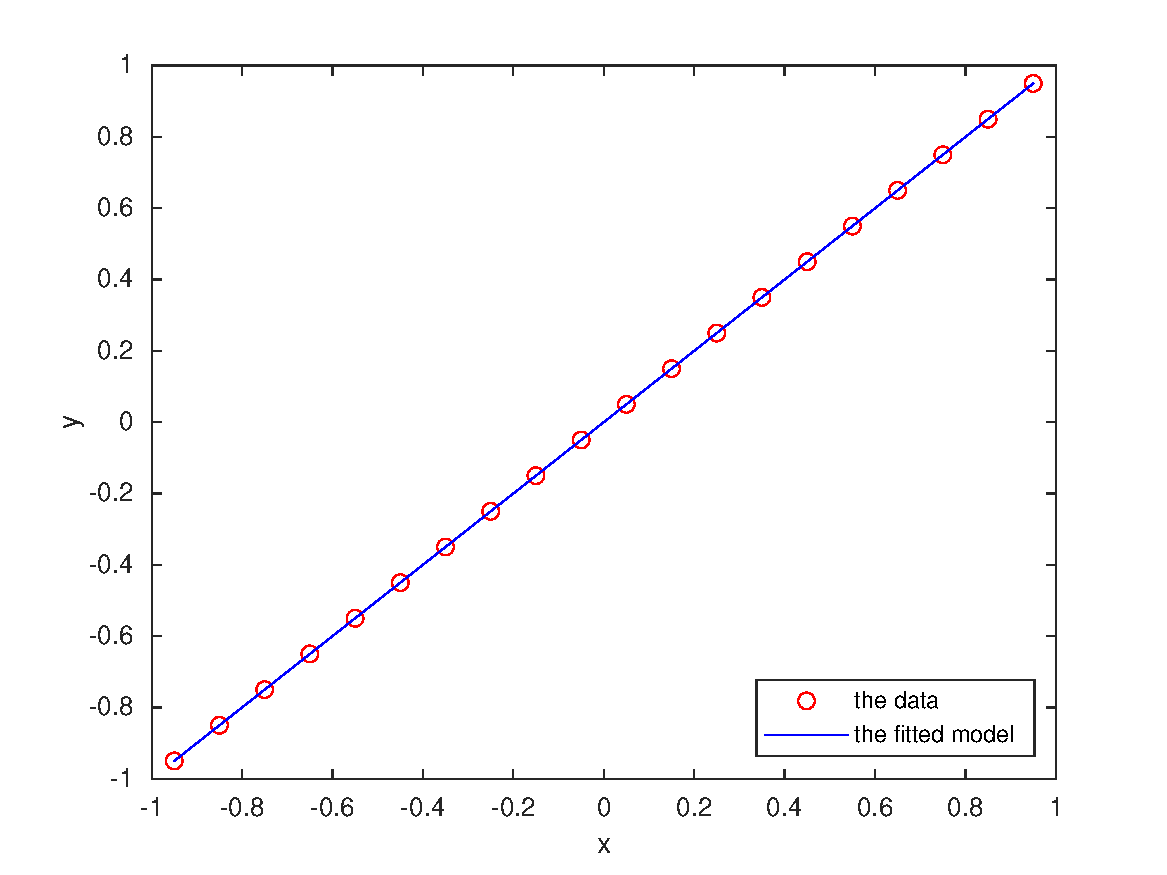
\includegraphics[width=6in, keepaspectratio]{hw3/hw3e51.pdf}
    \label{fig:hw3e51}
\end{figure}

\begin{figure}[htb]
    \centering
    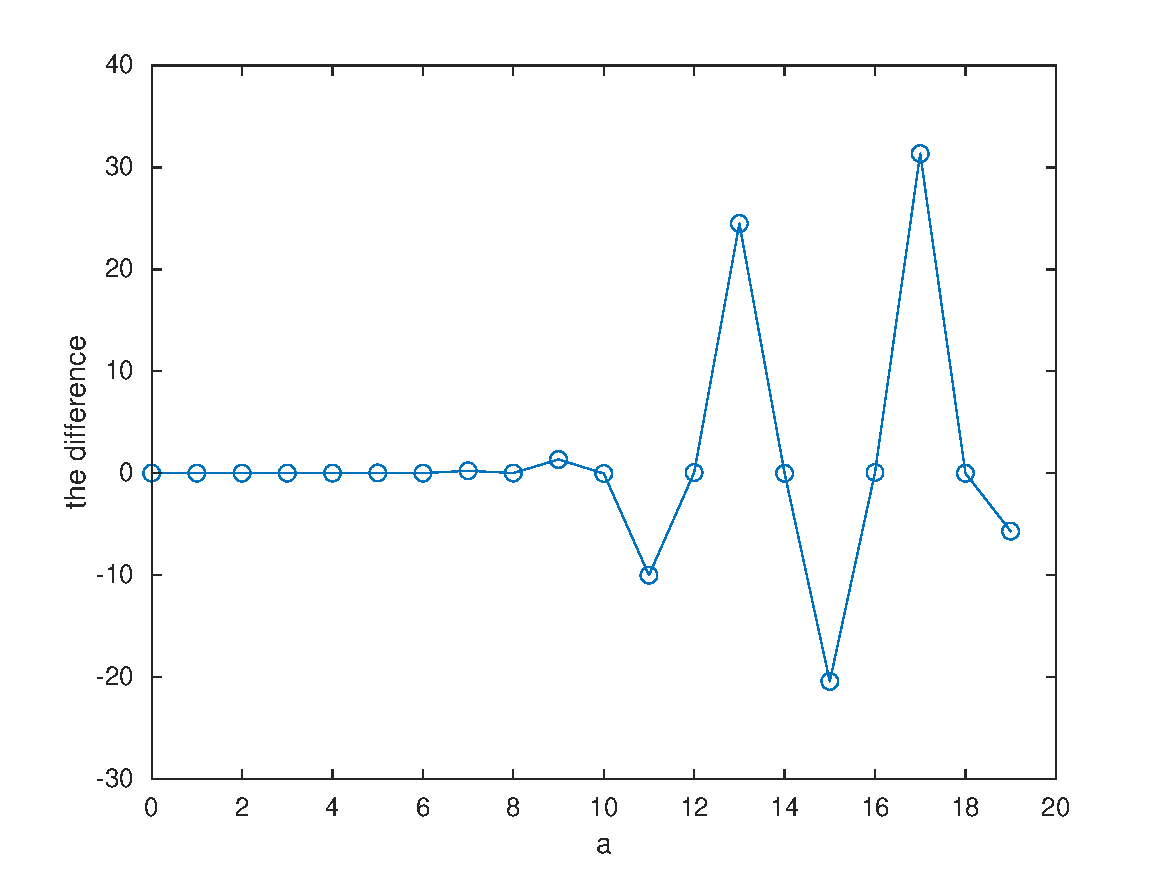
\includegraphics[width=6in, keepaspectratio]{hw3/hw3e52.pdf}
    \label{fig:hw3e52}
\end{figure}

\end{homeworkProblem}


\end{document}
